\documentclass[a4paper,12pt,openany]{report}
\usepackage{calc}

%\reversemarginpar \DeclareMathAlphabet{\mathpzc}{OT1}{pzc}{m}{it}
\usepackage{amsmath,amssymb,amsthm,wasysym}
%\textheight=24.7cm \textwidth=15cm \frenchspacing
\linespread{1.5}
%\usepackage[height=24.7cm, width=16cm, top=1.7cm, bottom=3.2cm, left=3.05cm, right=2.25cm]{geometry}
\usepackage[height=24.7cm, width=16cm, top=2.2cm, bottom=1.5cm, left=2.8cm, right=1.7cm]{geometry}
%\usepackage[height=23.8cm, width=15cm, top=2.5cm, bottom=3.5cm, left=3.5cm, right=2.5cm]{geometry}
%\usepackage[height=24.7cm, width=16cm, top=2.5cm, bottom=2.5cm, left=3.2cm, right=2.1cm]{geometry}
%\setlength{\oddsidemargin}{0.378in} 
%\setlength{\topmargin}{-0.015in}
%\setlength{\textheight}{23.80cm}
%\setlength{\textwidth}{15cm}
%\setlength{\marginparsep}{0pt}
%\setlength{\marginparwidth}{0.985in} 
\setcounter{table}{0}
\setcounter{page}{1}
\setcounter{section}{0}
\setcounter{figure}{0}

\newtheorem{theorem}{\textbf{Theorem}}[section]
\newtheorem{exodappl}{\textbf{Exercice d'application}}[section]
\newtheorem{solexodappl}{\textbf{Solution}}[section]
\newtheorem{properties}{\textbf{Properties}}[section]
\theoremstyle{plain}
\newtheorem{lemma}{\textbf{Lemma}}[chapter]
\theoremstyle{plain}
\newtheorem{proposition}{\textbf{Proposition}}[section]
\theoremstyle{plain}
\newtheorem{cla}{\textbf{Résultat}}[chapter]
\theoremstyle{plain}
\newtheorem{remark}{\textbf{Remark}}[section]
\newtheorem{property}{\textbf{Property}}[section]
\newtheorem{problem}{\textbf{Problème}}[section]
\theoremstyle{plain}
\newtheorem{rap}{\textit{Rappels}}[chapter]
\theoremstyle{plain}
\newtheorem{ob}{\textit{observation}}[chapter]
\theoremstyle{plain}
\newtheorem{exercise}{\underline{Exercice}}[chapter]
\newtheorem{solexo}{\underline{Exercice}}[chapter]
\newtheorem{definition}{\textbf{Definition}}[section]
\theoremstyle{plain}
\newtheorem{example}{\textbf{Example}}[section]
\theoremstyle{plain}
\newtheorem{corollary}{\textbf{Corollary}}[section]
\theoremstyle{plain}
%\newtheorem{prev}{\textbf{preuve}}[chapter]
\newenvironment{prevf}[1][\underline{Proof}]{\textbf{#1.} }{\ \rule{0.5em}{0.5em}}
\theoremstyle{plain}
\newtheorem{cor}{\textbf{Corollary}}[section]
\theoremstyle{plain}
\newcommand{\C}{\mathbb{C}}
\newcommand{\M}{\mathbb{M}}
\newcommand{\N}{\mathbb{N}}
\newcommand{\R}{\mathbb{R}}
\usepackage{tocloft}
%this is to change the name of the list of figures
\renewcommand*\listfigurename{LIST OF FIGURES}
%this is to change the name of the list of figures
\renewcommand*\listtablename{LIST OF TABLES}
%this is to change the name of the bibliography
\renewcommand*\bibname{\centerline{BIBLIOGRAPHY}}
%this is to center the liste of figures name
\renewcommand{\cftloftitlefont}{\vspace*{-2.4cm}\hspace*{\fill}\normalsize\bfseries}
\renewcommand{\cftafterloftitle}{\vspace*{-1.3cm}\hspace*{\fill}}
%this is to have in the list of figure the notation figure number: title of the figure. E.g figure 1: my figure
\newlength\mylen
\renewcommand\cftfigpresnum{\figurename\enspace}
\renewcommand\cftfigaftersnum{:}
\settowidth{\mylen}{\cftfigpresnum\cftfigaftersnum}
\addtolength{\cftfignumwidth}{\mylen}

%this is to center the table of contents name
\renewcommand{\cfttoctitlefont}{\vspace*{-2.4cm}\hspace*{\fill}\normalsize\bfseries}
\renewcommand{\cftaftertoctitle}{\vspace*{-1.8cm}\hspace*{\fill}}

%this is to center the table of tables name
\renewcommand{\cftlottitlefont}{\vspace*{-2.4cm}\hspace*{\fill}\normalsize\bfseries}
\renewcommand{\cftafterlottitle}{\vspace*{-1.3cm}\hspace*{\fill}}
%this is to have in the list of table the notation table number: title of the table. E.g table 1: my table
%\newlength{\mylen}
\renewcommand\cfttabpresnum{\tablename\enspace}
\renewcommand\cfttabaftersnum{:}
\settowidth{\mylen}{\cfttabpresnum\cfttabaftersnum}
\addtolength{\cfttabnumwidth}{\mylen}



\usepackage{graphicx}
\usepackage{multirow}
\usepackage[latin1]{inputenc}
\usepackage{t1enc}
\usepackage{float}

%this is to have the notation figure1/table1 instead of figure1.1/table1.1 under chapter1
\usepackage{chngcntr}
\counterwithout{figure}{chapter}
\counterwithout{table}{chapter}

%for matlab code 
\usepackage[T1]{fontenc}
\usepackage{xcolor,times}
% % % % % % % % % % % % inclure la source % % % % % % % % % %
\usepackage{listings}
\newcommand*\styleC{\fontsize{9}{10pt}\usefont{T1}{ptm}{m}{n}\selectfont }
\newcommand*\styleD{\fontsize{7}{10pt}\usefont{T1}{pag}{m}{n}\itshape\selectfont }
\makeatletter
\lstset{language=matlab}
\edef\Motscle{emph={\lst@keywords}}
\expandafter\lstset\expandafter{ %
}
\makeatother
\definecolor{Ggris}{rgb}{0.45,0.48,0.45}
\lstset{emphstyle=\rmfamily\color{blue}, %les mots reserves de matlab en bleu
	basicstyle=\styleC,
	keywordstyle=\ttfamily,
	commentstyle=\color{blue}\styleD, %commentaire en gris
	numberstyle=\tiny\color{red},
	numbers=left,
	numbersep=10pt,
	lineskip=0.7pt,
	showstringspaces=false}
% % inclure le fichier source
\newcommand{\FSource}[1]{ %
	\lstinputlisting[texcl=true]{#1}
}

\usepackage{titlesec}
\titlespacing{\chapter}{0pt}{0pt}{0.5 cm}
\titleformat{\chapter}[display]{\vspace*{-0.8cm}\normalfont\large\bfseries\centering}{\chaptertitlename\hspace*{0.2cm} \thechapter}{5pt}{\large \centering}
\titleformat{\section}{\normalfont\large\bfseries}{\thesection}{1em}{}
\titleformat{\subsection}{\normalfont\large\bfseries}{\thesubsection}{1em}{}
%\textwidth=15cm
%\textheight=24,7cm
%hoffset=-2.5cm
\tolerance=9000
\hbadness=9000
\pretolerance=2500
\usepackage{pdfpages}
\renewcommand{\thepage}{\roman{page}}

\begin{document}
		
	
	\begin{titlepage}\thispagestyle{empty}
		\begin{center}
			\fontsize{14}{20}{\bf { UNIVERSITY OF BAMENDA} }
			\begin{flushleft}
				$\begin{tabular}{ccc}
				%	\ & \ & \ \\
				\multirow{3}{6.50cm}{\centering \fontsize{14}{6.5cm}{\bf  {FACULTY OF SCIENCE } } }& \multirow{3}{3.00cm}{
\includegraphics[height=3.00cm,width=3.3cm]{logo.png} } & \multirow{3}{6.50cm}{\centering	\fontsize{14}{6.5}{\bf { DEPARTMENT OF MATHEMATICS AND COMPUTER SCIENCE}  }}
				%	\Large{\bf  {HIGHER TEACHER TRAINING COLLEGE (HTTC) BAMBILI} } & 
\includegraphics[height=4.00cm,width=4.01cm]{logo.png} & 	\Large{\bf {MATHEMATICS DEPARTMENT}  }\\
				%\ & 
\includegraphics[height=4.00cm,width=4.01cm]{logo.png} & \ \\
				\end{tabular}$
			\end{flushleft}
			\vspace*{3cm}
			\begin{center}
				\begin{tabular}{|c|}
					\hline
					\nolinebreak \ \\
					\multirow{1}{14.00cm}{\centering \large $\boldmath${ \bf
							{POST-MODEL SELECTION AND MEASUREMENT ERROR IN HIGH-DIMENSIONAL DATA
					}}}\\
					\nolinebreak \ \\
						\nolinebreak \ \\
					%	\nolinebreak \ \\
					\hline
				\end{tabular}
			\end{center}
		\end{center}
		\vspace*{-0.3cm}
		\begin{center}
			\textit{\normalsize
				A dissertation submitted to the Department Of Mathematics and Computer Science of the
				Faculty of Science, in the University of Bamenda in partial fulfillment of the requirements for the
				award of the Masters Degree (MSc.) in Probability and Statistics.
				 }
		\end{center}
		
		%	\vspace*{1cm}
		\begin{center}
			\ \\
			By\\ 
			\large{\textbf{YIMTSOP ROLEX BRICE} }\\
			\fontsize{12}{14}{UBa18SP045 }\\
			( BSc. in Applied Mathematics)\\
			\vspace*{2cm}
			\fontsize{12}{14}{ Supervisor} \\
			\fontsize{12}{14}\linespread{1.5}\selectfont {\textbf{PROF. NGUEFACK-TSAGUE GORGES }}\\
			\fontsize{12}{14}{ Co-Supervisor} \\
			\fontsize{12}{14}\linespread{1.5}\selectfont {\textbf{Dr. KUM CLETUS KWA }}\\
			%(Senior Lecturer - University of BUEA)\\
			\vspace*{3cm}
			\fontsize{12}{14}{\textbf{DECEMBER, 2020}}
		\end{center}
	\end{titlepage}
	
	\begin{titlepage}
		\vspace*{23.5cm}
		\begin{center}
			\textcopyright\ \ Copyright by \textbf{YIMTSOP ROLEX BRICE}, 2020\\
			All Rights Reserved.
		\end{center}
	\end{titlepage}
	
	
	
	
	%\maketitle
	\chapter*{DECLARATION}\addcontentsline{toc}{chapter}{DECLARATION}
	\pagenumbering{roman}
	\noindent
	I, \textbf{YIMTSOP ROLEX BRICE},
	 registration $N^{\circ}$: \textbf{UBa18SP045}, Department of Mathematics and Computer Science in the Faculty of Science of the University of Bamenda hereby declare
	that, this dissertation titled: "\textbf{Post-Model Selection and Measurement Error in High-Dimensional Data}" is my original work. It has not been presented in any application for a degree or any academic pursuit. I have sincerely acknowledged all borrowed ideas nationally and internationally through citations.
	\vspace{2cm}
	
	\[\text{Date:\underline{\hspace*{5cm}} \hspace*{3.5 cm} Signature\underline{\hspace*{5cm}}}\] 		


	
\chapter*{CERTIFICATION}\addcontentsline{toc}{chapter}{CERTIFICATION}
\noindent
This is to certify that this research titled: "\textbf{Post-Model Selection and Measurement Error in High-Dimensional Data}" is the original work of \textbf{ YIMTSOP ROLEX BRICE}. This work is submitted in partial fulfillment of the requirements for the award of a Master's degree (MSc.) in mathematics, Faculty of Science of the University of Bamenda, Cameroon.


\vspace*{2 cm}
\begin{center}
	\begin{tabular}{cccccc}
	\underline{\hspace*{5cm}}\\ 
	\textbf{	Prof. NGUEFACK-TSAGUE GEORGES}\\
	(Supervisor) 	
	\end{tabular}
	
\end{center}
\vspace*{3 cm}
\begin{center}
	\begin{tabular}{cccccc}
		\underline{\hspace*{6cm}}&\hspace*{3cm}& \underline{\hspace*{6cm}}\\
		\textbf{Dr. FELIX CHE SHU} & \hspace*{1cm}& \textbf{Prof. TABOT CHARLES TABOT} \\
		(Head of Department) &  \hspace*{3cm} & (Dean)  \\	
	\end{tabular}	
\end{center}
Having met the stipulated requirements, the dissertation has been accepted by the Postgraduate School
\vspace*{2 cm}
\begin{center}
		\begin{tabular}{cccccc}
	Date:	\underline{\hspace*{5cm}}  \hspace*{5.2cm}   \underline{\hspace*{5cm}} \\
	\hspace*{5.8cm}   \hspace*{5.2cm}   \textbf{The General Coordinator}\\
	\hspace*{5.8cm}  \hspace*{4.8cm}   \textbf{Postgraduate School} \\	
		\end{tabular}
\end{center}


	

\chapter*{DEDICATION}\addcontentsline{toc}{chapter}{DEDICATION}

\begin{center}
		This dissertation is lovingly dedicated to my beloved mother, \textbf{DJIMELI Philomene} and father, \textbf{TAGUELA Fran\c{c}ois}. Their support, encouragement, and constant love have sustained me throughout my life.

\end{center}

\chapter*{ACKNOWLEDGEMENTS}\addcontentsline{toc}{chapter}{ACKNOWLEDGEMENTS}
\noindent
\begin{itemize}
\item[]	This dissertation would not have been written without the help and encouragement of many people. I
	take this opportunity to highlight some of them.
	
	\item[] First and foremost, I would like to express my gratitude to my supervisor, \textbf{Prof. NGUEFACK-TSAGUE GORGES}.
		His true researcher attitude and his careful reading of many manuscripts that I gave him, which is illustrated in being very receptive to new ideas, his passion
		for science, which results in being very knowledgeable and hardworking scientist, and his sense of
		responsibility, which results in easy reachability makes him an ideal supervisor and which I hope to continue to explore the joy of scientific research.
		\item[] I express my sincere thanks to my co-supervisor \textbf{Dr. KUM Cletus Kwa} Head of Department of Mathematics of the higher teacher training college of the University of Bamenda for his encouragements and for the continuous support of my dissertation study. 
		
		  \item[] My special appreciation
		is expressed to \textbf{ Dr. SHU FELIX CHE} the head of the department of Mathematics and Computer
		Science,this work would not be possible
		without his patience, motivation, enthusiasm, and immense knowledge.  
		
		\item[] I also express my sincere thanks to \textbf{Dr. FOUTSA Emmanuel} senior lecturer of the University of Bamenda for all his advice in my live and his encouragements and orientation in my future mathematics field during this year. 
		\item[] To all the lecturers of Mathematics and Computer Science Department. I thank \textbf{Prof. MARTIN NDUMU, Prof. FONO LOUIS, Dr. PATRICE NDAMBOMVE, Prof. MAURICE NDIKONTAR, Dr. VUKENKENG ANDREW WUJUNG}, which through the relevance of their lesson offered a formation of quality to me.
		\item[] I gratefully appreciate my beloved parents for their
		love, sacrifices and encouragement. I would like to express my special thanks to my friends for
		their suggestions and encouragement. Finally, I would like to thank every one, who supported
		me, but I did not mention above.
	\end{itemize}
	
\chapter*{ABSTRACT}\addcontentsline{toc}{chapter}{ABSTRACT}
\noindent
Much theoretical and applied work has been devoted to high-dimensional clean data. However, in many problems involving generalised linear models, we often face corrupted data in many applications where measurement errors cannot be ignored. It is thus necessary to extend regularisation methods, that can handle the situation where the number of covariates $p$ is much larger than the sample size $n$, to the case in which covariates are also mismeasured. When the number of covariates $p$ exceeds the sample size $n$,
regularised methods like the Lasso or Dantzig selector are required. Several recent papers have studied methods which correct for measurement error in the Lasso or Dantzig selector for linear models in the $p > n$ setting, but many of them require knowledge about the measurement error structure or the covariance matrix of the measurement error. We study a correction for generalised
linear models, based on Rosenbaum and Tsybakov's matrix uncertainty selector in which the measurement error and its covariance matrix are not known and have to be estimated from data and focus on variable selection in which the evaluation is based on simulations. In our simulation studies, we focus on linear, logistic
and Poisson regression with measurement error. The proposed methods outperform the
standard lasso with respect to covariate selection, by reducing
the number of false positives. We also investigate a general procedure that utilizes the recently proposed Imputational-regularized Optimization algorithm for high-dimensional data with measurement error, which we implement for continuous, binary, and count response variable.\\
	\underline{\textbf{Keywords}}: generalised linear model, high-dimensional data, measurement error, matrix uncertainty selector
\chapter*{R\'ESUM\'E}\addcontentsline{toc}{chapter}{R\'ESUM\'E}
\noindent
Beaucoup de travaux th\'{e}oriques et appliqu\'{e}s on \'{e}t\'{e} consacr\'{e}s aux donn\'{e}es propres de grande dimension. Cependant, dans de nombreux probl\`{e}mes impliquant des mod\`{e}les lin\'{e}aires g\'{e}n\'{e}ralis\'{e}s, nous sommes souvent confront\'{e}s \`{a} des donn\'{e}es corrompues dans de nombreuses applications o\`{u} les erreurs de mesure ne peuvent \^{e}tre ignor\'{e}es. il est donc n\'{e}cessaire d'\'{e}tendre les m\'{e}thodes de r\'{e}gularisation, qui peuvent g\'{e}rer la situation o\`{u} le nombre de covariables $p$ est beaucoup plus grand que la taille de l'\'{e}chantillon $n$, au cas o\`{u} les covariables sont \'{e}galement mal mesur\'{e}es. Lorsque le nombre de covariables $p$ d\'{e}passe la taille de l'\'{e}chantillon $n$, des m\'{e}thodes r\'{e}gularis\'{e}es comme le Lasso ou le Dantzig selecteur sont requises. Plusieurs articles r\'{e}cents ont \'{e}tudi\'{e} des m\'{e}thodes qui corrigent l'erreur de mesure dans le Lasso ou le Dantzig selecteur pour les mod\`{e}les lin\'{e}aires dans le r\'{e}glage $p>n$, mais beaucoup d'entre eux n\'{e}cessitaient des connaissances sur la structure d'erreur de mesure ou la matrix de covariance de la mesure d'erreur. Nous \'{e}tudions une correction pour les mod\`{e}les lin\'{e}aires g\'{e}n\'{e}ralis\'{e}s, bas\'{e}e sur le s\'{e}lecteur d'incertitude matricielle de Rosenbaum et Tsybakov dans lequel l'erreur de mesure et sa matrice de covariance ne sont pas connues et doivent \^{e}tre estim\'{e}es \`{a} partir de donn\'{e}es et se concentrer sur les mod\`{e}les de regression lin\'{e}aire, logistique et Poisson avec erreur de mesure. La m\'{e}thodes propos\'{e}es surpassent le Lasso standard en ce qui concerne la s\'{e}lection des covariables, en r\'{e}duisant le nombre de faux positifs. Nous \'{e}tudions \'{e}galement une proc\'{e}dure g\'{e}n\'{e}rale qui utilise l'algorithme d'optimisation r\'{e}gularis\'{e} par imputation r\'{e}cemment propos\'{e} pour les donn\'{e}es de grande dimension avec erreur de mesure, que nous impl\'{e}mentons pour la variable de r\'{e}ponse continue, binaire et de comptage.
	\\ 
	\underline{\textbf{Mots cl\'es}}: mod\`{e}le lineaire g\'{e}n\'{e}ralis\'{e}, donn\'{e}es de grandes dimensions, matrice de selection d'incertitude, erreur de mesure   

	
	\newpage
	\renewcommand{\contentsname}{TABLE OF CONTENTS}
	\tableofcontents
	\addcontentsline{toc}{chapter}{TABLE OF CONTENTS}        
	
	\newpage
	\listoftables\addcontentsline{toc}{chapter}{LIST OF TABLES}
	
	\newpage
	\listoffigures\addcontentsline{toc}{chapter}{LIST OF FIGURES}
	
		\chapter*{LIST OF ABBREVIATIONS}\addcontentsline{toc}{chapter}{LIST OF ABBREVIATIONS}
	\noindent
	HD : High-dimensional\\
	i.i.d : Independent and Identically Distributed\\
AIC : AKAIC Information Criterion\\
BIC : Bayesian Information Criterion\\
DIC : Deviance Information Criterion\\
FIC : Focused Information Criterion\\
MUS : Matrix Uncertainty Selector\\
GMUL : Generalised Matrix Uncertainty Lasso\\
GLM : Generalised linear Model\\
GLMs : Generalised linear Models\\
GMUS : Generalised Matrix Uncertainty Selector\\
GDS : Generalised Dantzig Selector\\
DS : Dantzig Selector\\
Id : Identity\\
Lasso : Least Absolute Shrinkage Operator\\
HDME : High-Dimensional with Measurement Error.\\
L : Lasso	
	\chapter{GENERAL INTRODUCTION}
	\pagenumbering{arabic}
	\section{Background and Motivation}
	\noindent
Model selection is the task of selecting a statistical model from a set of candidate models, given data. More precisely, estimating the performance of different models in order to choose the (approximate) best one. Traditional subset selection methods combined with variable selection criteria, such as AIC, BIC, DIC, FIC are used to select a model among candidate models. These criteria may perform well in the relatively low dimensional space. However, these methods suffer from expensive computational cost and model instability for high-dimensional data (High-dimensional refers to the situations where the number covariates or predictors is much larger than the sample size). Recently, various regularisation methods through penalisation of parameters have been proposed for variable selection in high-dimensional regression analysis. Examples include the least absolute shrinkage and selection operator (LASSO) of Tibshirani (1996), the smoothly clipped absolute deviation (SCAD) (Zou and Li 2008), the least-angle regression (LARS) algorithm (Efron et al. 2004), the elastic net (Zou and Zhang 2009), the Dantzig selecor (DS) (Candes and Tao 2007), among others. \\

There are certain areas of classical statistics where model selection has played an important role, for example, linear regression and time series. In both sets of problems one asks essentially the same question: Which variables in a linear relation or linear predictor are worth keeping? This becomes a model selection problem if one identifies each set of retained variables with a model.	
It would be naive to expect the best results by including all the variables in one\textquoteright s model. One way of seeing this is to note that it violates the fundamental scientific principle of parsimony, which requires that of all the models that explain the data well, one should choose the simplest.
Generalised linear models (GLMs) is another area in classical statistics where model selection is popular. In these applications it is used as an alternative to classical testing of hypothesis.\\

However, in practical applications, high-dimensional data analyses have to take into account measurement error in the covariates. It is thus necessary to extend regularisation methods, that can handle the situation where the number of covariates say, $p$ is larger than the sample size say, $n$, to the case in which covariates are also mismeasured. In reality, the data in most applications are subject to at leat some measurement error. Some examples are, gene expression microarrays subject to various sources of systematic and random error, which are noisy versions of the true gene expressions in the patients (Rocke and Durbin, 2001); food frequency questionnaires used in epidemiologic studies, in which subjects are asked about their food consumption and it is well known that people don't always tell the truth in survey (Kipnis t al., 2003); sensor network data also tend to be noisy, due to measurement error or sensor failure (Bertrand and Moonen, 2011).\\

In classical regression context, when $p<n$ and standard methods can be applied, it is well known that measurement error in the covariates will lead to bias in estimation of parameters and to loss of power (Carroll et al., 2006). Many correction methods are available to reduce this bias, but they generally need information about the measurement error structure. We refer to (belloni et al., 2014; Chen and Caramanis, 2013; Datta and Zou, 2015; Liang and Li, 2009; Loh and wainwright, 2012; Ma and Li, 2010; Rosenbaum and Tsybakov, 2010, 2013; Sorensen et al., 2015; Zhu et al., 2011). Typically, this require validation data or replicate measurements of the covariates in order to estimate the measurement error distribution. Most of these techniques require knowledge of the measurement error distribution or at least the covariance matrix of the measurement error, yielding estimators with good theoretical properties. However, in practice this will almost always be unknown, and estimation of the covariance matrix of the measurement error can be computationally expensive or even unfeasible when the number of variables $p$ increases. Exceptions are the matrix uncertainty selector (MUS)(Rosenbaum and tsybakov, 2010), sparse total least squares (Zhu et al., 2011), and the modified orthogonal matching pursuit (Chen and Caramanis, 2013), that can account for measurement error without additional information about the measurement error structure, but sacrifice some statistical properties to get this robustness. The latter methods hence have a practical advantage in many applications, and in particular, they have been shown to yield fewer false positive selections than the standard Lasso and Dantzig selector. Kaul et al. (2016) proposed a two-stage non-penalised corrected least squares, which performs variable selection in the first step, and estimates the regression coefficient of the selected variables in the next step.\\

The methods proposed for dealing with measurement error in penalised regression all
focus on linear regression, with the exception of Ma and Li (2010); Sorensen et al. (2015).
Considering the importance and general applicability of GLMs, it is therefore of interest
to develop penalised regression methods for GLMs which do not require an esimate of the
measurement error distribution, and recover the linear regression framework as a special
case. In this work, we investigate the generalised MUS (GMUS), based on a Taylor expansion
of the GLM mean function around the true, but unknown, values of the covariates. The
GMUS can be computed using an iterative reweighing procedure, and when the Taylor
expansion is truncated at first order, each step of this procedure requires solving a linear
program. We also develop a generalised matrix uncertainty lasso (GMUL), which is a lasso type analog of the DS-based GMUS. The GMUL estimate can also be computed using an
iterative reweighing procedure, in which an inner coordinate descent loop has to be run
until a stopping criterion is met in each step of the algorithm. In simulation experiments
with linear, logistic and Poisson regression, the GMUL and GMUS with the first order Taylor
approximation are shown to give very promising covariate selection results compared to
the lasso and the GDS, by detecting considerably fewer false positives (FPs) at similar
numbers of true positives (TPs). We also investigate the extension to the Imputation-Regularized Optimization (IRO) algorithm for common types of generalised linear models in the presence of measurement error.

\section{Objectives of work}
The main goal of this work is to look into penalised regression for generalised linear models (GLMs) with measurement error
and to compare some of these methods in a practical context, where the distribution and
the variance of the measurement error is unknown and need to be estimated from data.
The comparison will be based on simulations, and the focus will be on the linear
regression model, logistic model and poisson models with additive measurement error.
\section{Layout of work}
The work is organised as follows. We start in Section 2 with a brief preliminary and notations. In Section 3, we give an overview of the models and methods that we will investigate and
their theoretical properties. Section 4 describes the simulation setups with real data example and results, and Section 5 is devoted to the interpretation of the results
and some final conclusions and recommendation
\chapter{Preliminaries}
\section{Generalised Linear Model}
Most of the commonly used statistical distributions, e.g. Normal,
Binomial, Gamma, Poisson and Inverse-Gaussian are members of the exponential family of
distributions. The advantage of expressing diverse families of distributions in the common exponential form
is that general properties of exponential families can then be applied to the individual cases.
\begin{definition}
	Let $y=(y_1, y_2,\dots, y_n)^T$ be the response variable, $X=(x_1, x_2, \dots, x_n)^T$ the covariate vector, and $\beta = (\beta_0,\ldots,\beta_p)^T$ be the vector of coefficients. The distribution of $Y$ belongs to the exponential family of distributions if its density can be written in the form:
	\begin{equation}\label{ec21}
	f_Y(y,\theta,\phi)=\exp\left\lbrace\frac{y\theta-b(\theta)}{a(\phi)}+c(y,\phi)\right\rbrace,
	\end{equation}
	where $a(.)$, $b(.)$, and $c(.)$ are known functions that vary from one exponential family to another, $\phi$ is the dispersion parameter and $\theta$ is the vector of linear predictors given by
	\begin{equation}\label{ec22}
	\theta_i=\mathbf{x}_i^T\beta=\beta_0+\beta_1x_{i1}+\dots+\beta_px_{ip}, \ \ i=1,2,\dots, p,
	\end{equation} 
	
\end{definition}
A generalised linear model can be briefly characterised by the following three components
\begin{enumerate}
	\item Independent random variables $y_1, y_2,\dots, y_n$ with expected value $\mathbb{E}(y_i)=\mu_i$ and density function from the exponential family.\\
	\item A linear predictor $\theta_i$ given by equation $(\ref{ec22})$\\
	\item A link function, $g$, that describes how $\mathbb{E}(y_i)=\mu_i$ relates to $\theta_i$
	\begin{eqnarray}
	g(\mu_i)=\theta_i
	\end{eqnarray}
\end{enumerate}
\begin{lemma}
	The following equality can be verified using likelihood function of the exponential familly given in equation $(\ref{ec21})$
	\begin{equation}
	\left\lbrace\begin{array}{ll}
	\mathbb{E}(Y) =& b^{'}(\theta)=\mu(\theta)\\
	var(Y) =& b^{''}(\theta)\phi = V(\mu)\phi
	\end{array}\right.
	\end{equation}
\end{lemma}
The exponential family distributions with their link and mean functions are given in table 1.

\begin{table}\label{tc21}\centering
	\begin{tabular}{l|c|c}
		\hline
		Family & Link function $\theta_i=g(\mu_i)$ & Mean function $\mu_i = g^{-1}(\theta_i)$\\
		\hline
		Gaussian & $ Id(\mu_i) =\mu_i$ & $\theta_i$\\
		
		Binomial & $Logit(\mu_i)=\log_e\left(\frac{\mu_i}{1-\mu_i}\right)$ & $\frac{1}{1+e^{-\theta_i}}$\\
		Poisson & $\log_e(\mu_i)$ & $e^{\theta_i}$\\
		Gamma & $\mu_i^{-1}$ & $\theta_i^{-1}$\\
		Inverse-Gaussian & $\mu_i^{-2}$ & $\theta_i^{-1/2}$\\
		\hline
	\end{tabular}
	\caption{Link and mean functions for exponential family distributions}
\end{table}
The regularized GLM aime to minimize, with respect to $\beta$, the objective:
\begin{equation}
Q(\beta; X, y, \lambda) = \mathcal{L}(y; x, \beta) + P(\beta;\lambda),
\end{equation}
where $\mathcal{L}(y; x, \beta)$ is the negative log-likelihood function and $P(\beta;\lambda)$ is the penalty function on the coefficients. In clean HD data, the Lagrangian form of the Lasso (Tibshirani, 1996) estimates of $\beta$ can be obtained by minimizing the negative log-likelihood of equation $(\ref{ec21})$ in the following nonsmooth convex optimization problem.

\begin{equation}\label{ec23}
\hat{\beta}_{L} = \underset{\beta}{argmin}\left[\frac{-1}{n}\sum_{i=1}^{n}\left\lbrace y_i\theta_i-b\left(\theta_i\right)\right\rbrace + \lambda||\beta||_1\right]
\end{equation}
where $\theta_i=\mathbf{x}_i^T\beta$, $\lambda > 0$, is the regularisation parameter and $||\cdot||_p$ denotes the $\ell_p$ norm for vectors and matrices for $1\leq p\leq\infty$. The GDS however solves:
\begin{equation}\label{ec24}
\hat{\beta}_{DS} = \underset{\beta}{argmin}\left[||\beta||_1 : \underset{1\leq j\leq p}{\max} \left|\frac{1}{n}\sum_{i=1}^{n}x_{ij}\left\lbrace y_i-\mu\left(\theta_i\right)\right\rbrace\right| \leq \lambda\right]
\end{equation}

\subsection{Logistic Regression}
In some regression situations, the response variable y has only two possible outcomes, for example, high blood pressure or low blood pressure, developing cancer
of the esophagus or not developing it, whether a crime will be solved or not
solved, document classification (presence versus absence). In such cases, the outcome $y$ can be coded as $0$ or $1$ and we wish to
predict the outcome (or the probability of the outcome) on the basis of one or
more $x$'s.\\

To illustrate a linear model in which y is binary, consider the model:
\begin{equation}\label{eq:logistic1}
y_i = \beta_0+\beta_1x_{i1}+\ldots+\beta_px_{ip} + \epsilon_{i}, \ \ \ y_i=1,1; \ \ i=1,2,\ldots,n.
\end{equation}
Since $y_i$ is $0$ or $1$, the mean $\mathbb{E}(y_i)$ for each $x_{ip}$ becomes the proportion of observations at
$x_{ip}$ for which $y_i = 1$. This can be expressed as
\begin{eqnarray}\label{eq:logistic2}
\begin{array}{lcl}
\mathbb{E}(y_i)& = &\mathbb{P}(y_i=1)=p_i,\\
1-\mathbb{E}(y_i)& = &\mathbb{P}(y_i=0)= 1-p_i.
\end{array}
\end{eqnarray}
The distribution $\mathbb{P}(y_i=0)= 1-p_i$ and $\mathbb{P}(y_i=1)=p_i$ in \eqref{eq:logistic2} is known as the
Bernoulli distribution. By \eqref{eq:logistic1} and \eqref{eq:logistic2}, and the fact that $\beta_0+\beta_1x_{i1}+\ldots+\beta_px_{ip}=\mathbf{x}^T\beta$, with $\mathbf{x}_i=(1,x_i1,\ldots,x_ip)$, $\beta= (\beta_0,\ldots,\beta_p)$, we have
\begin{equation}\label{eq:logistic3}
\mathbb{E}(y_i) = p_i = \mathbf{x}_i^T\beta.
\end{equation}
To obtain optimal estimators of $\beta$, we could use generalised least-squares
estimators
\begin{equation}
\hat{\beta} = \left(\mathbf{X}^T\mathbf{V}^{-1}\mathbf{X}\right)^{-1}\mathbf{X}^T\mathbf{V}^{-1}y
\end{equation}
Since $\mathbb{E}(y_i)=p_i$ is a probability, it is limited by $0 \leq p_i\leq 1$. If we fit \eqref{eq:logistic3}
by generalised least squares to obtain
\begin{equation}
\hat{p}_i = \mathbf{x}_i^T\hat{\beta}
\end{equation}
then $\hat{p}_i$ may be less than $0$ or greater than $1$ for some values of $\mathbf{x}_i^T$. A model for $\mathbb{E}(y_i)$
that is bounded between $0$ and $1$ and reaches $0$ and $1$ asymptotically (instead of
linearly) would be more suitable. A popular choice is the logistic regression model.
\begin{equation}
p_i = \mathbb{E}(y_i) = \frac{e^{\mathbf{x}_i^T\mathbf{\beta}}}{1+e^{\mathbf{x}_i^T\mathbf{\beta}}},
\end{equation}
which can be linearlized by the simple transform
\begin{equation}\label{eq:logistic4}
\ln\left(\frac{p_i}{1-p_i}\right) = \mathbf{x}_i^T\mathbf{\beta}.
\end{equation}
Given the logistic model \eqref{eq:logistic4}, the negative log-likelihood with Lasso regularization takes the form
\begin{eqnarray}
&-& \frac{1}{n}\sum_{i=1}^{n}\left[y_i\ln p_i+(1-y_i)\ln(1-p_i)\right] +\lambda||\beta||_1\\
 &=& -\frac{1}{n}\sum_{i=1}^{n}\left[y_i\mathbf{x}_i^T\mathbf{\beta}-\ln\left(1+e^{\mathbf{x}_i^T\mathbf{\beta}}\right)\right] +\lambda||\beta||_1
\end{eqnarray}
\subsection{Poisson Regression}
If the response $y_i$ in a regression model is a count, the Poisson regression model may
be useful. The Poisson probability distribution is given by
\begin{equation}\label{eq:poisson1}
f(y)=\frac{\mu^ye^{-\mu}}{y!},\ \ \  y=0,1,2,\ldots.
\end{equation}
The Poisson regression model is
\begin{equation}
y_i = \mathbb{E}(y_i)+\epsilon_{i}, \ \ \ i=1,2,\ldots,n,
\end{equation}
where the $y_i$'s are independently distributed as Poisson random variables and $\mu_i = \mathbb{E}(y_i)$ is a function of $\mathbf{x}_i^T\beta = \beta_0 +\beta_1x_{i1}+\ldots+\beta_px_{ip}$.\\
 Given the logistic model \eqref{eq:poisson1}, the negative log-likelihood with Lasso regularization takes the form
 \begin{equation}
 -\frac{1}{n}\sum_{i=1}^{n}\left[y_i\ln\left(\mathbf{x}_i^T\mathbf{\beta}\right)-\mathbf{x}_i^T\mathbf{\beta}-\ln\left(y!\right)\right] +\lambda||\beta||_1
 \end{equation}
\subsection{Linear Regression}
In the linear model 
\begin{equation}
y_i = X\beta + \epsilon,
\end{equation}
where the residual error $\epsilon$ is normally distributed with mean $0$ and variance $\sigma^2$, i.e., $\epsilon\AC N(0,\sigma^2)$. then $y\AC N(\mu,\sigma^2)$ with $\mu=X\beta$. The lasso (Tbshirani, 1994) estimates the regression coefficient vector by 
\begin{equation}
\hat{\beta} = \underset{\beta}{\arg\min}\frac{1}{2n}||y-X\beta||_2^2 + \lambda||\beta||_1.
\end{equation} 
The distribution of $y$ can be expression into the form of the exponential family as
\begin{eqnarray}
f(y,\theta,\phi) = \frac{1}{\sigma\sqrt{2\pi}}\exp\left\lbrace -\frac{1}{\sigma^2}(y-\mu)\right\rbrace
=\exp\left\lbrace\frac{y\theta-\theta^2/2}{\phi}-\frac{1}{2}\left[\frac{y^2}{\phi}+\ln(2\pi\phi)\right]\right\rbrace,
\end{eqnarray}
where $\theta = \mu$, $\phi=\sigma^2$, $a(\phi)=\phi$, $b(\theta)=\theta^2/2$ and $c(y,\phi) = -1/2\left[y^2/\phi+\ln(2\pi\phi)\right]$.\\
Similarly, the Poisson, gamma, Binomial and inverse-Gaussian families can all be put into the form of exponential family using the results given in Table 2.\\
\begin{table}\label{tc21}\centering
	\begin{tabular}{l|c|c|c}
		\hline
		Family & $a(\phi)$ & $b(\theta)$ & $c(y,\phi)$\\
		\hline

		Gaussian & $\phi$ & $\theta^2/2$ &$-1/2\left[y^2/\phi+\ln(2\pi\phi)\right]$\\
		
		Binomial & $1/n$ & $\log_e(1+e^{\theta})$ & $\log_e(_{ny}^n)$\\
		Poisson & 1 & $e^{\theta}$ & $-\log_ey!$\\
		Gamma & $\phi$ & $-\log_e(-\theta)$ & $-\phi^{-2}\log_e(y/\phi)-\log_ey-\log_e\Gamma(\phi^{-1})$\\
		Inverse-Gaussian & $\phi$ & $-\sqrt{-2\theta}$ & $-1/2\left[\log_e(\pi\phi y^3)+1/(\phi y)\right]$\\
		\hline
	\end{tabular}
	\caption{a(), b(.) and c(.) functions for exponential family distributions}
\end{table}
where $\Gamma(.)$ is the gamma function define as $\Gamma(x)=\int_{0}^{\infty}e^{-t}t^{x-1}dt$.
\section{Convex Optimisation Problem}
A mathematical optimization problem, has the form
\begin{equation}\label{eq:opti}
\text{minimised} \ \ f(x) \ \ \text{subject to} \ \ g_i(x)\leq b_i, \ \ i=1,\ldots,m,
\end{equation}
were the vector $x = (x_1,\ldots, x_n)$ is the optimization variable of the problem, the
function $f : \mathbb{R}^n\to\mathbb{R}$ is the objective function, the functions $g_i : \mathbb{R}^n\to\mathbb{R}$,
$i = 1,\ldots, m$, are the (inequality) constraint functions, and the constants $b_1,\ldots, b_m$
are the limits, or bounds, for the constraints. A vector $x^*$ is called optimal, or a
solution of the problem \eqref{eq:opti}, if it has the smallest objective value among all vectors
that satisfy the constraints: for any $z$ with $g_1(z) \leq b_1,\ldots,g_m(z) \leq b_m$, we have
$f(z) \geq f(x^*)$. The optimization problem \eqref{eq:opti} is called a linear program if the objective
and constraint functions $f,g_1,\ldots,g_m$ are linear.\\
An important class of optimization problems involves convex constraint and convex objective functions. A convex optimization problem is one in which the objective and
constraint functions are convex
\subsection{Convex Optimality for Differentiable Problems}
\begin{definition}
	A set $\mathcal{A}\subseteq\mathbb{R}$ is said to be convex if for all $\beta_1, \beta_2\in\mathcal{A}$ and all scalars $t\in\left[0,1\right]$, the vector $t\beta_1+(1-t)\beta_2\in\mathcal{A}$. A function $f : \mathbb{R}^p\to\mathbb{R}$ is is said to be convex if for any two vectors $\beta_1, \beta_2\in\mathbb{R}^p$ and any scalar $t\in(0,1)$, we have
	\begin{equation}
	f(t\beta_1+(1-t)\beta_2) \leq tf(\beta_1) + (1-t)f(\beta_2)
	\end{equation}
\end{definition}
Consider the constrained optimization problem
\begin{equation}\label{eq:convexopt}
\underset{\beta\in\mathbb{R}^p}{\text{minimize}}f(\beta)\ \ \ \ \text{such that}\ \ \beta\in\mathcal{A},
\end{equation}
where $f : \mathbb{R}^p\to\mathbb{R}$ is a convex objective function to be minimised, and $\mathcal{A}\subset\mathbb{R}^p$ is a convex constraint set. When the objective function $f$ is differentiable, then a necessary and sufficient condition for a vector $\beta^*\in\mathcal{A}$ to be a global optimum is that
\begin{equation}\label{eq:gradient}
\left\langle\bigtriangledown f(\beta^*), \beta-\beta^*\right\rangle\geq 0, \ \ \ \text{for all}\ \ \beta\in\mathcal{A}
\end{equation}
where $\bigtriangledown$ is the gradient. In particular, when $\mathcal{A}=\mathbb{R}^p$, the problem \eqref{eq:convexopt} is unconstrained and then the first order condition \eqref{eq:gradient} reduces to the classical zero-gradient condition $\bigtriangledown f(\beta^*) = 0$.
\begin{proposition}
	For any convex function $g : \mathbb{R}^p\to\mathbb{R}$, the sublevel set $\left\lbrace\beta\in\mathbb{R}^p| g(\beta)\leq 0\right\rbrace$ is a convex set.
\end{proposition}
The convex optimization problem
\begin{equation}\label{eq:convexopt2}
\underset{\beta\in\mathbb{R}^p}{\text{minimize}}f(\beta)\ \ \ \ \text{such that}\ \ g_j(\beta)\leq 0\ \ \text{for} \ j=1,2,\ldots,m,
\end{equation}
where $g_j,j=1,2,\ldots,m$ are convex functions that express constraints to be satisfied, is an instance of the general program \eqref{eq:convexopt}.
An important function associated with the problem \eqref{eq:convexopt} is the Lagrangian $L : \mathbb{R}^p\times\mathbb{R}_+^m\to\mathbb{R}$, defined by
\begin{equation}
L(\beta;\lambda) = f(\beta)+\sum_{j=1}^{m}\lambda_jg_j(\beta).
\end{equation}
The nonnegative weights $\lambda\geq 0$ are known as the Lagrange multipliers; the purpose of the multiplier $\lambda_j$ is to impose a penalty whenever the constraint $g_j(\beta) \leq 0$ is violated. Indeed, if we allow the multipliers to be chosen optimally, then we recover the original program \eqref{eq:convexopt2}, since
\begin{eqnarray}
\underset{\lambda\geq 0}{\sup}L(\beta;\lambda) = \left\lbrace\begin{array}{ll}
f(\beta) & \text{if}\ \ g_j(\beta)\leq 0 \ \ \text{for all} \ j=1,2,\ldots,m\\
+\infty & \text{otherwise},
\end{array}\right.
\end{eqnarray}
Then if $f^*$ denote the optimal value of the optimization problem \eqref{eq:convexopt2}, we have
\begin{equation}
 f^*=\underset{\beta\in\mathbb{R}^p}{\inf}\underset{\lambda\geq 0}{\sup}L(\beta;\lambda).
\end{equation}
\begin{definition}{(The KKT condition)}
	The Karush-Kuhn-Tucker conditions relate the optimal Lagrange multiplier vector $\lambda^*\geq 0$, also known as the dual vector, to the optimal primal vector $\beta^*\in\mathbb{R}^p$:
	\begin{enumerate}
		\item \textit{Primal feasibility}: $g_j(\beta^*)\leq 0$ for all $j=1,2,\ldots,m$.
		\item \textit{Complementary slackness}: $\lambda_j^*g_j(\beta^*) =0$ for all $j=1,2,\ldots,m$.
		\item \textit{Lagrange condition}: the pair $(\beta^*,\lambda^*)$ satisfies the condition
		\begin{equation}\label{eq:Lagrange}
		0=\bigtriangledown_{\beta}L(\beta^*;\lambda^*) = \bigtriangledown f(\beta^*)+\sum_{j=1}^{m}\lambda_j^*\bigtriangledown g_j(\beta^*).
		\end{equation}
	\end{enumerate}
\end{definition}
The KKT conditions are necessary and sufficient condition for $\beta^*$ to be a global optimum.
\subsection{Convex Optimality for Nondifferentiable Function}
In practice, many optimization problems arising in statistics involve convex but nondifferentiable objective functions. 
\begin{example}
	The $\ell_1$-norm $g(\beta)=||\beta||_1=\sum_{j=1}^{p}|\beta_j|$ is a convex function, but it fails to be differentiable at any point where at least one coordinate $\beta_j$ is equal to zero. For such problems, the optimality conditions \eqref{eq:gradient} and \eqref{eq:Lagrange} are not directly applicable, since they involve gradients of the objective and constraint functions.
\end{example} 
\begin{definition}
	Let $f : \mathbb{R}^p\to\mathbb{R}$ be a convex function. a vector $z\in\mathbb{R}^p$ is said to be a subgradient of $f$ at $\beta_0$ if
	\begin{equation}
	f(\beta) \geq f(\beta_0) + \left\langle z, \beta-\beta_0\right\rangle \ \ \ \text{for all} \ \ \beta\in\mathbb{R}^p.
	\end{equation}
\end{definition}
The set of all subgradients of $f$ at $\beta_0$ is called the sub-differential, denoted by $\partial f(\beta_0)$. At points of nondifferentiability, the subdifferential is a convex set containing all possible subgradients.
\begin{example}
	For the absolute value function $f(\beta) = |\beta|$, we have
	\begin{eqnarray}\label{eqa:absolutevalue}
	\partial f(\beta) = \left\lbrace\begin{array}{ll}
	+1 & if\ \  \beta > 0\\
	-1 & if\ \  \beta < 0\\
	\left[-1,+1\right] & if\ \ \beta = 0
	\end{array}\right.
	\end{eqnarray}
\end{example}
We frequently write $z\in sign(\beta)$ to mean that $z$ belongs to sub-differential of the absolute value function at $\beta$. Recall the convex optimization problem \eqref{eq:convexopt2}, and assume that one or more of the functions $\left\lbrace f, g_j\right\rbrace$ are convex but nondifferentiable. In this case, the zero-gradient Lagrangian condition \eqref{eq:Lagrange} no longer makes sense. But under mild conditions on the functions, the generalised KKT theory can still be applied using the modified condition
\begin{equation}\label{eq:subgradient}
0 \in\partial f(\beta^*) + \sum_{j=1}^{m}\lambda_j^*\partial g_j(\beta^*),
\end{equation}
In which we replace the gradients in the KKT condition \eqref{eq:Lagrange} with the subdifferentials.
\begin{example}
	Suppose that we want to solve a minimisation problem of the form \eqref{eq:convexopt2} with a convex and differentiable objective function $f$, and a single constraint specified by $g(\beta) = \sum_{j=1}^{p}|\beta_j| - R$ for some positive constant $R$. Thus, the constraint $g(\beta)\leq 0$ is equivalent to requiring that $\beta$ belongs to an $\ell_1$-ball of radius $R$. Recalling the form of the subdifferential \eqref{eqa:absolutevalue} for the absolute value function, condition \eqref{eq:subgradient} becomes
	\begin{equation}
	\bigtriangledown f(\beta^*) + \lambda^*z^* = 0,
	\end{equation}
	where the subgradient vector satisfies $z_j^*\in sign(\beta_j^*)$ for each $j=1,2,\ldots,p$.
\end{example}
When the objective function $f$ takes the form of the squared error $f(\beta) = \frac{1}{2n}||y-X\beta||_2^2$, this condition is equivalent to
\begin{equation}
-\frac{1}{n}\left\langle x_j, y-X\beta\right\rangle + \lambda s_j=0, \ \ \ j=1,2,\ldots,p.
\end{equation}
where $s_j= sing(\beta_j)$ if $\beta_j\neq 0$ and some value lying in $\left[-1,1\right]$ otherwise.
\subsection{Some Inequalities}
\begin{definition}(Triangle Inequality)
for $x, y\in\mathbb{C}$,
\begin{equation}
|x+y|\leq |x|+|y|.
\end{equation}	
\end{definition}
More generally, for $x_i\in\mathbb{C}$, $i=1,\ldots,n$, the generalised triangle inequality for finite sums is given by
\begin{equation}
\left|\sum_{i=1}^{n}x_i\right| \leq \sum_{i=1}^{n}|x_i|.
\end{equation}
\begin{definition}(H\"{o}lder's Inequality)
	For $x_i, y_i\in\mathbb{C}$, $i=1,\ldots,n$, if $1\leq p<\infty$ and $1/p + 1/q = 1$ then the H\"{o}lder's Inequality for finite sums is given by
	\begin{equation}\label{eq:holder}
	\sum_{i=1}^{n}|x_iy_i| \leq \left(\sum_{i=1}^{n}|x_i|^p\right)^{1/p} +\left(\sum_{i=1}^{n}|x_i|^q\right)^{1/q}
	\end{equation}
\end{definition}
In the particular case where $p=q=2$, the inequality \eqref{eq:holder} becomes the well known, Schwartz's inequality.
\chapter{Model Setup and Methods}

\section{Measurement error in covariates}

 In the additive measurement error model, the unobservable variable $X$ is altered by adding random measurement error $U$, so what we observe is
\begin{equation}
w_i=x_i+u_i,\ \ \ for \ \ i=1,\dots, n.
\end{equation} 
 This can be re-formulated in matrix notation as:
\begin{equation}
W = X + U,
\end{equation}
where $U$ ia an $n\times p$ random noise matrix with covariance matrix $\Sigma_U$. 
If the covariates are measured with error, and we end up working with a contaminated covariate $W$, the naive Lasso estimate obtained by simply replacing $X$ by $W$ in $(\ref{ec23})$ can be systematically biased (Rosenbaum and Tsybakov, 2010).\\

A key assumption is that the measurement error is standardized to have $0$ mean and unit variance; i.e., for $j=1,2,\ldots,p$,
\begin{equation}\label{eq:standardized}
\frac{1}{n}\sum_{i=1}^{n}w_{ij} = 0, \ \ \ \frac{1}{n}\sum_{i=1}^{n}w_{ij}^2 = 1. 
\end{equation}

Define the vector $\epsilon = (\epsilon_1, \dots, \epsilon_n)^T$, and the generalised residual $\epsilon_i = y_i-\mu(\theta_i)$, $i=1,\dots, n$ Without measurement error, $\beta$ is contained in the feasible set of the GDS if $\lambda$ is chosen such that
\begin{equation}\label{ec25}
\frac{1}{n}||X^T\epsilon||_{\infty}\leq \lambda,
\end{equation}
where $||.||_{\infty}$ is the maximum component norm, holds (Antoniadis et al., 2010; Candes and Tao, 2007). Hence, for any GDS solution $\hat{\beta}_{DS}$ as well as the for the true regression coefficients $\beta$, the maximum correlation of any covariate with the residual is bounded by $\lambda$. This also means that under restricted eigenvalue conditions, $\hat{\beta}_{DS}$ and $\beta$ are close, and that their maximun possible distance increases in $\lambda$. Hence, a natural starting point for a theoretical analysis is to assume that the bound $(\ref{ec25})$ holds (B$\ddot{u}$hlmann and van de Geer, 2011, p. 103).  Both of the previous selection methods assume the true covariates of the measurement to be observed.  This is often not the case. When $X$ is measured with error, the true coefficient vector $\beta$ may not be part of the feasible set, even when $\lambda$ is set to its theoretically optimal value in $(\ref{ec25})$. The reason is that $\lambda$ is a bound on the residual of model, while in the case of measurement error, a bound on the measurement matrix $U$ is also needed. The Matrix Uncertainty Selector (MUS) first introduced by Rosenbaum and Tsybakov (2010) as a modification of the Dantzig Selector for data with measurement error. In the special case of linear regression, Rosenbaum and Tsybakov (2010) developed the MUS by adding to the DS a new parameter $\delta$ that bounds the magnitude of the measurement error. They showed that when:
\begin{equation}\label{eq:bound}
\frac{1}{n}||W^T\epsilon||_{\infty}\leq \lambda \ \ \text{and} \ \  ||U||_{\infty} \leq \delta,
\end{equation}
the vector of the true parameters $\beta$ is a feasible solution of the MUS, defined as follows:
\begin{equation}
\hat{\beta}_{MUS} = \underset{\beta}{argmin}\left[||\beta||_1 :  \frac{1}{n}||W^T(y-W\beta)||_{\infty} \leq \lambda + \delta||\beta||_1\right]. 
\end{equation}
Note that the MUS does not require an estimate of the measurement error covariance matrix $\Sigma_U$. This
might be a practical advantage in some cases, when an estimate of $\Sigma_U$ is hard to obtain. It is worth noting that the estimation error bounds for the MUS do not go to zero when $n\to\infty$. This is the price to pay for not knowing the measurement error distribution. The choice of the unknown tuning parameters in the MUS is from a practical point of view
not trivial. We chose to select the parameter $\lambda$ through cross-validation. In particular we
used the parameter selected by cross-validation of the naive lasso, i.e. the lasso
of y on W.
The choice of the parameter $\delta$ is critical. Low values of $\delta$ implies that the measurement
error is not taken into account, while big values will overweight this effect. According to "elbow rule" (Rosenbaum and Tsybakov, 2010), the choice of the parameter value $\delta$ can be chosen where the curve starts to level off. This is not always easy in practice, but in the following plot, figure $\ref{fc21}$ a value between $0.05$ and $0.1$ may be reasonable.

\begin{figure}\label{fc21}
	\centering
	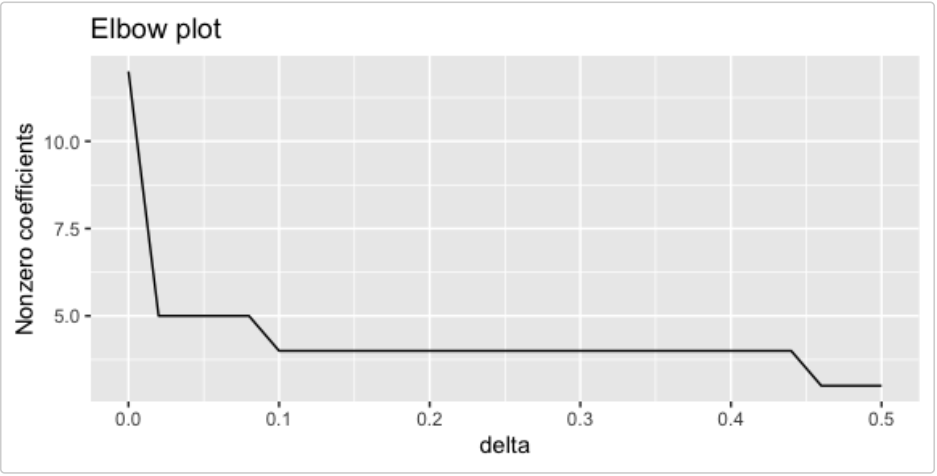
\includegraphics[width=0.9\linewidth]{F1ElbowPlot}
	\caption{Elbov plot for HDME setting with $n=50$, $p=1000$}
\end{figure}

\section{Generalised Matrix Uncertainty Selector}

The Generalised Matrix Uncertainty Selector (GMUS) is an extension of the MUS to generalised linear models, introduced by Sorensen et al. (2018). 
\begin{proposition}\label{prop31}
	
GMUS is defined as the solution to the optimization problem:
\begin{equation}\label{eq:boundGMUS}
\hat{\beta}_{GMUS} = \underset{\beta}{argmin}\left[||\beta||_1 :  \frac{1}{n}||W^T(y-\mu(W\beta))||_{\infty} \leq \lambda + \sum_{r=1}^{R}\frac{\delta^r}{r!\sqrt{n}}||\beta||_{1}^{r}||\mu^{(r)}(W\beta)||_2\right] 
\end{equation}
where $\mu^{(r)}(.)$ is the $r$th derivative of the vector valued mean function $\mu(.)$ of the generalised linear model.
\end{proposition}
\begin{proof}
	It follows from the Taylor series expansion of the mean function $\mu(\theta_i)=\mu(x_i^T\beta)$ around the scalar point $\mathbf{w}_i^T\boldsymbol{\beta}$ that
	\begin{equation*}
	\mu\left(\mathbf{x}_{i}^{T}\boldsymbol{\beta}\right) =  \sum_{r=0}^{\infty} \frac{\mu^{(r)}\left( \mathbf{w}_{i}^{T}\boldsymbol{\beta}\right)}{r!} \left(-\mathbf{u}_{i}^{T}\boldsymbol{\beta}\right)^{r}.
	\end{equation*}
	Which implies that
	\begin{equation*}
	\mu\left(\mathbf{w}_{i}^{T}\boldsymbol{\beta}\right) = \mu\left(\mathbf{x}_{i}^{T}\boldsymbol{\beta}\right) - \sum_{r=1}^{\infty} \frac{\mu^{(r)}\left( \mathbf{w}_{i}^{T}\boldsymbol{\beta}\right)}{r!} \left(-\mathbf{u}_{i}^{T}\boldsymbol{\beta}\right)^{r}.
	\end{equation*}
	This gives, for $j=1,\dots,p$,
	\begin{align*}
	\frac{1}{n}\left|\sum_{i=1}^{n} w_{ij}\left\{y_{i} - \mu\left(\mathbf{w}_{i}^{T}\boldsymbol{\beta} \right) \right\} \right| &=& 
	 \frac{1}{n}\left|\sum_{i=1}^{n} w_{ij}\left\{\epsilon_{i}+ \sum_{r=1}^{\infty} \frac{\mu^{(r)}\left( \mathbf{w}_{i}^{T}\boldsymbol{\beta}\right)}{r!} \left(-\mathbf{u}_{i}^{T}\boldsymbol{\beta}\right)^{r}\right\} \right| \\
	 &\leq&
	 \frac{1}{n}\left|\sum_{i=1}^{n} w_{ij}\epsilon_{i} \right| + \frac{1}{n}\left|\sum_{i=1}^{n} w_{ij} \sum_{r=1}^{\infty} \frac{\mu^{(r)}\left( \mathbf{w}_{i}^{T}\boldsymbol{\beta}\right)}{r!} \left(-\mathbf{u}_{i}^{T}\boldsymbol{\beta}\right)^{r} \right|\\
	 & \leq& 
	 \lambda + \frac{1}{n}\left|\sum_{i=1}^{n} w_{ij} \sum_{r=1}^{\infty} \frac{\mu^{(r)}\left( \mathbf{w}_{i}^{T}\boldsymbol{\beta}\right)}{r!} \left(-\mathbf{u}_{i}^{T}\boldsymbol{\beta}
	\right)^{r} \right| \\
	&\leq& 
	  \lambda + \frac{1}{n}\sum_{i=1}^{n}\left| w_{ij} \sum_{r=1}^{\infty} \frac{\mu^{(r)}\left( \mathbf{w}_{i}^{T}\boldsymbol{\beta}\right)}{r!} \left(-\mathbf{u}_{i}^{T}\boldsymbol{\beta}\right)^{r} \right|,
	\end{align*}
	where we inserted $\epsilon_{i} = y_{i} - \mu\left(\mathbf{w}_{i}^{T}\boldsymbol{\beta}\right)$ in the first step, we used the triangle inequality in the second step, we inserted the left bound in \eqref{eq:bound} in the third step, and finally used the generalised triangle inequality. Next, we have
	\begin{align*}
	\frac{1}{n}\sum_{i=1}^{n}\left| w_{ij} \sum_{r=1}^{\infty} \frac{\mu^{(r)}\left( \mathbf{w}_{i}^{T}\boldsymbol{\beta}\right)}{r!} \left(-\mathbf{u}_{i}^{T}\boldsymbol{\beta}\right)^{r} \right| &\leq& \frac{1}{n}\left(\sum_{i=1}^{n} w_{ij}^{2} \right)^{\frac{1}{2}} \left[\sum_{i=1}^{n} \left\{ \sum_{r=1}^{\infty} \frac{\mu^{(r)}\left( \mathbf{w}_{i}^{T}\boldsymbol{\beta}\right)}{r!} \left(-\mathbf{u}_{i}^{T}\boldsymbol{\beta}\right)^{r}\right\}^{2} \right]^{\frac{1}{2}}\\
	 & =& 
	 \frac{1}{\sqrt{n}} \left[\sum_{i=1}^{n} \left\{ \sum_{r=1}^{\infty} \frac{\mu^{(r)}\left( \mathbf{w}_{i}^{T}\boldsymbol{\beta}\right)}{r!} \left(-\mathbf{u}_{i}^{T}\boldsymbol{\beta}\right)^{r}\right\}^{2} \right]^{\frac{1}{2}},
	\end{align*}
	where we used Schwartz's inequality in the first step and the assumption \eqref{eq:standardized} that the covariates are standardized to have mean zero and unit variance in the second step. We now note that the last term above is the $\ell_{2}$-norm $\|\mathbf{v}\|_{2}$ of a vector $\mathbf{v} \in \mathbb{R}^{n}$ with elements
	\begin{equation*}
	v_{i} =  \sum_{r=1}^{\infty} \frac{\mu^{\left(r\right)}
		\left( \mathbf{w}_{i}^{T}\boldsymbol{\beta}\right)}{r!} \left(-\mathbf{u}_{i}^{T}\boldsymbol{\beta}\right)^{r},\quad i=1,\dots,n.
	\end{equation*}
	We thus have
	\begin{align*}
	\frac{1}{\sqrt{n}} \left[\sum_{i=1}^{n} \left\{ \sum_{r=1}^{\infty} \frac{\mu^{(r)}\left( \mathbf{w}_{i}^{T}\boldsymbol{\beta}\right)}{r!} \left(-\mathbf{u}_{i}^{T}\boldsymbol{\beta}\right)^{r}\right\}^{2} \right]^{\frac{1}{2}} &\leq& 
	 \frac{1}{\sqrt{n}} \sum_{r=1}^{\infty} \left[ \sum_{i=1}^{n}\left\{\frac{\mu^{(r)}\left( \mathbf{w}_{i}^{T}\boldsymbol{\beta}\right)}{r!} \right\}^{2}\left(-\mathbf{u}_{i}^{T}\boldsymbol{\beta}\right)^{2r} \right]^{\frac{1}{2}}\\
	 & \leq&
	 \frac{1}{\sqrt{n}} \sum_{r=1}^{\infty} \left[ \sum_{i=1}^{n}\left\{\frac{\mu^{(r)}\left( \mathbf{w}_{i}^{T}\boldsymbol{\beta}\right)}{r!} \right\}^{2} \left\|\mathbf{u}_{i}\right\|_{\infty}^{2r} \left\|\boldsymbol{\beta}\right\|_{1}^{2r}\right]^{\frac{1}{2}}\\
	 & \leq & \sum_{r=1}^{\infty}\frac{\delta^{r}\left\|\boldsymbol{\beta}\right\|_{1}^{r}}{r!\sqrt{n}}  \left[ \sum_{i=1}^{n}\left\{\mu^{(r)}\left( \mathbf{w}_{i}^{T}\boldsymbol{\beta}\right) \right\}^{2}  \right]^{\frac{1}{2}}\\
	 & =&  \sum_{r=1}^{\infty}\frac{\delta^{r}\left\|\boldsymbol{\beta}\right\|_{1}^{r}}{r!\sqrt{n}} \left\|\boldsymbol{\mu}^{(r)}\left(\mathbf{W}\boldsymbol{\beta} \right) \right\|_{2} ,
	\end{align*}
	where we used the triangle inequality in the first step, H\"older's inequality in the second step, and finally used the right bound in \eqref{eq:bound} in the second last step.
	
	Putting the pieces together, it follows that
	\begin{align*}
	\frac{1}{n}\left|\sum_{i=1}^{n} w_{ij}\left\{y_{i} - \mu\left(\mathbf{w}_{i}^{T}\boldsymbol{\beta} \right) \right\} \right| \leq  \lambda +\sum_{r=1}^{\infty}\frac{\delta^{r}}{r!\sqrt{n}} \left\|\boldsymbol{\beta}\right\|_{1}^{r} \left\|\boldsymbol{\mu}^{(r)}\left(\mathbf{W}\boldsymbol{\beta} \right) \right\|_{2} 
	\end{align*}
	for $j=1,\dots,p$, which proves that the result.
\end{proof}
 $R$ is a parameter controlling the number of Taylor expansion terms which are included. When $R\to\infty$, the true solution is a member of the feasible set given that the bounds
\begin{equation}
\frac{1}{n}||W^T\epsilon||_{\infty}\leq \lambda \ \ \text{and} \ \  ||U||_{\infty} \leq \delta,
\end{equation}
hold. For computational reason in the rest of this work, we set $R=1$. When $R=1$, the GMUS can be solved using a sequence of linear programming problems on the same form as the MUS, with an iterative reweighing algorithm.
\subsection{Iterative Reweighing Algorithm for GMUS}
We assume that the contaminated current estimate of the linear predictor for sample $i$ after completing the $k$th iteration is $\theta_i^{W(k)} = w_i^T\beta^{(k)}$.
We define the adjusted dependent covariate as
\begin{equation}\label{ec26}
z_i = \theta_i^{W(k)} + \left[y_i-\mu\left(\theta_i^{W(k)}\right)\right]\left[\mu'\left(\theta_i^{W(k)}\right)\right]^{-1}, \ \ \ i=1,2,\dots,n.
\end{equation}
We define a weight vector for each term in the Taylor expansion with $R$ terms as
\begin{equation}\label{ec27}
V^{(r)} = \left[\mu^{(r)}\left(\theta_1^{W(k)}, \dots, \theta_n^{W(k)}\right)\right]^T.
\end{equation}
We introduce the matrix $\tilde{W}\in\mathbb{R}^{n\times p}$ and the vector $\tilde{z}\in\mathbb{R}$ as
\begin{equation}\label{ec28}
\tilde{w_{ij}} = w_{ij}\sqrt{V_i^{(1)}}, \ \  \ \ \tilde{z}_i = z_i\sqrt{V_i^{(1)}}, \ \  \ \ r=1, 2, \ldots, R, \ \ i=1, 2, \ldots, n, \ \ j=1, 2, \ldots, p.
\end{equation}
The next iterate $\beta^{(k+1)}$ is now given by
\begin{equation}\label{ec29}
\hat{\beta}_{GMUS}^{(k+1)} = \underset{\beta}{argmin}\left[||\beta||_1 :  \frac{1}{n}||\tilde{W}^T(\tilde{z}-\tilde{W}\beta)||_{\infty} \leq \lambda + \sum_{r=1}^{R}\frac{\delta^r}{r!\sqrt{n}}||\beta||_{1}^{r}||V^{(r)}||_2\right].
\end{equation}
 The iterative reweighing procedure for GMUS is then define as
\begin{table}
	\begin{tabular}{l}
		\hline
		\textbf{Algorithm 1} Iterative reweighing procedure for GMUS\\
		\hline
		input: initial estimate $\beta^{(0)}$, $k=0$, $R\in\mathbb{N}$,\\
		\textbf{repeat}\\
		Compute $z$, $V^{(r)}$, $\tilde{W}$, $\tilde{z}$ and $\beta^{(k+1)}$, as given in equation $(\ref{ec26})$, $(\ref{ec27})$, $(\ref{ec28})$ and $(\ref{ec29})$.\\
		$k\leftarrow k+1$\\
		\textbf{until} $||\beta^{(k)}-\beta^{(k+1)}||< \epsilon_{tol}$\\
		\textbf{return} $\hat{\beta}_{GMUS}=\beta^{(k)}$\\
		\hline
	\end{tabular}
\caption{Iterative reweighing procedure for GMUS}
\end{table}
\begin{theorem}
The solution obtained in algorithm $1$ satisfied the inequality \eqref{eq:boundGMUS} in proposition $\ref{prop31}$
\end{theorem}
\begin{proof}
	Consider a fixed point of the Algorithm $1$. At a fixed point, $\beta^{\left(k+1\right)} = \beta^{\left(k\right)}$. It follows that
	\begin{align*}
	z_{i} = \mathbf{w}_{i}^{T}\boldsymbol{\beta}^{(k+1)} + \left[y_{i} - \mu\left\{ \mathbf{w}_{i}^{T}\boldsymbol{\beta}^{(k+1)}\right\}\right]\mu^{\prime}\left\{ \mathbf{w}_{i}^{T}\boldsymbol{\beta}^{(k+1)} \right\}^{-1}, ~i=1,\dots,n
	\end{align*}
	and
	\begin{align*}
	\mathbf{V}^{(r)} = \left[\mu^{(r)}\left\{ \mathbf{w}_{1}^{T}\boldsymbol{\beta}^{(k+1)} \right\} , \dots, \mu^{(r)}\left\{\mathbf{w}_{n}^{T}\boldsymbol{\beta}^{(k+1)} \right\}\right]^{T},
	\end{align*}
	and accordingly,
	\begin{align*}
	\tilde{w}_{ij} = \sqrt{\mu^{\prime}\left\{ \mathbf{w}_{i}^{T}\boldsymbol{\beta}^{(k+1)} \right\} }w_{ij}, \quad \tilde{z}_{i} =\sqrt{\mu^{\prime}\left\{ \mathbf{w}_{i}^{T}\boldsymbol{\beta}^{(k+1)} \right\}}z_{i}.
	\end{align*}
	Inserting this into the constraint set in \eqref{ec29}, we get for the left-hand side
	\begin{align*}
	&\tilde{\mathbf{W}}^{T}\left(\tilde{\mathbf{z}} - \tilde{\mathbf{W}}\boldsymbol{\beta}^{(k+1)}\right)  = 
	\sum_{i=1}^{n} \tilde{w}_{ij} \left(\tilde{z}_{i} - \sum_{l=1}^{p} \tilde{w}_{il}\beta_{l}^{(k+1)}\right) = \\
	&\sum_{i=1}^{n} \sqrt{\mu^{\prime}\left\{ \mathbf{w}_{i}^{T}\boldsymbol{\beta}^{(k+1)} \right\} }w_{ij} \left(\sqrt{\mu^{\prime}\left\{ \mathbf{w}_{i}^{T}\boldsymbol{\beta}^{(k+1)} \right\}}z_{i}  - \sum_{l=1}^{p} \sqrt{\mu^{\prime}\left\{ \mathbf{w}_{i}^{T}\boldsymbol{\beta}^{(k+1)} \right\} }w_{ij} \beta_{l}^{(k+1)} \right) = \\
	&\sum_{i=1}^{n} \mu^{\prime}\left\{ \mathbf{w}_{i}^{T}\boldsymbol{\beta}^{(k+1)} \right\}  w_{ij}\left(z_{i} - \mathbf{w}_{i}^{T}\boldsymbol{\beta}^{(k+1)}\right) = \\
	&\sum_{i=1}^{n} \mu^{\prime}\left\{ \mathbf{w}_{i}^{T}\boldsymbol{\beta}^{(k+1)} \right\}  w_{ij}\left(\mathbf{w}_{i}^{T}\boldsymbol{\beta}^{(k+1)} + \left[y_{i} - \mu\left\{ \mathbf{w}_{i}^{T}\boldsymbol{\beta}^{(k+1)}\right\}\right]\mu^{\prime}\left\{ \mathbf{w}_{i}^{T}\boldsymbol{\beta}^{(k+1)} \right\}^{-1} - \mathbf{w}_{i}^{T}\boldsymbol{\beta}^{(k+1)}\right) = \\
	&\sum_{i=1}^{n} w_{ij} \left(y_{i} -  \mu\left\{ \mathbf{w}_{i}^{T}\boldsymbol{\beta}^{(k+1)}\right\}\right) = \\
	&\mathbf{W} \left(\mathbf{y} - \boldsymbol{\mu}\left\{\mathbf{W}\boldsymbol{\beta}^{(k+1)} \right\} \right).
	\end{align*}
	For the right-hand side of the inequality in \eqref{ec29}, we get
	\begin{align*}
	\lambda + \sum_{r=1}^{R}\frac{\delta^{r}}{r! \sqrt{n}} \left\|\boldsymbol{\beta}^{(k+1)}\right\|_{1}^{r}\left\| \mathbf{V}^{(r)}\right\|_{2} = \lambda + \sum_{r=1}^{R}\frac{\delta^{r}}{r! \sqrt{n}} \left\|\boldsymbol{\beta}^{(k+1)}\right\|_{1}^{r}\left\| \boldsymbol{\mu}^{(r)}\left\{\mathbf{W}\boldsymbol{\beta}^{(k+1)} \right\}\right\|_{2} .
	\end{align*}
	It follows that at any fixed point of Algorithm $1$, 
	\begin{align*}
	&\boldsymbol{\beta}^{(k+1)} = \\ 
	&\text{arg}\underset{\boldsymbol{\beta}}{\text{min}}\left\{ \left\| \boldsymbol{\beta}\right\|_{1}: \frac{1}{n}\left\|\tilde{\mathbf{W}}^{T}\left(\tilde{\mathbf{z}} - \tilde{\mathbf{W}}\boldsymbol{\beta}\right) \right\|_{\infty} \leq \lambda + \sum_{r=1}^{R} \frac{\delta^{r} }{r! \sqrt{n}} \left\|\boldsymbol{\beta}\right\|_{1}^{r}\left\| \mathbf{V}^{(r)}\right\|_{2}\right\} = \\
	&\text{arg}\underset{\boldsymbol{\beta}}{\text{min}}\left\{ \left\| \boldsymbol{\beta}\right\|_{1}: \frac{1}{n}\left\|\mathbf{W} \left(\mathbf{y} - \boldsymbol{\mu}\left\{\mathbf{W}\boldsymbol{\beta} \right\} \right) \right\|_{\infty} \leq \lambda + \sum_{r=1}^{R}\frac{\delta^{r}}{r! \sqrt{n}} \left\|\boldsymbol{\beta}\right\|_{1}^{r}\left\| \boldsymbol{\mu}^{(r)}\left\{\mathbf{W}\boldsymbol{\beta} \right\}\right\|_{2}\right\}.
	\end{align*}
	Thus, any fixed point of Algorithm $1$ is a solution to the original problem \eqref{eq:boundGMUS}.
\end{proof}
The computation of solution  \eqref{ec29} can be simplified 
 by introducing the auxiliary variable $\mathbf{u}\in\mathbb{R}^p$ (see, e.g., Candes and
Tao (2007, eq. (1.9)) or Boyd and Vandenberghe (2004, p. 617)) as follow 
\begin{align*}
&\text{mininimize } \mathbf{1}_{p}^{T} \mathbf{u} \text{ (with respect to } \mathbf{u}, \boldsymbol{\beta} \text{)}
\text{ subject to } -\mathbf{u} \leq \boldsymbol{\beta} \leq \mathbf{u}, \\
&-\sum_{r=1}^{R} \frac{\delta^{r}}{r! \sqrt{n}} \left(\mathbf{1}_{p}^{T} \mathbf{u}\right)^{r}\left\|\mathbf{V}^{(r)}\right\|_{2} \mathbf{1}_{p}+ \frac{1}{n}\tilde{\mathbf{W}}^{T}\tilde{\mathbf{W}} \boldsymbol{\beta} \leq  \lambda\mathbf{1}_{p} + \frac{1}{n}\tilde{\mathbf{W}}^{T} \tilde{\mathbf{z}},\text{ and}\\
&-\sum_{r=1}^{R} \frac{\delta^{r}}{r! \sqrt{n}} \left(\mathbf{1}_{p}^{T} \mathbf{u}\right)^{r}\left\|\mathbf{V}^{(r)}\right\|_{2}\mathbf{1}_{p}- \frac{1}{n}\tilde{\mathbf{W}}^{T}\tilde{\mathbf{W}} \boldsymbol{\beta} \leq 
\lambda \mathbf{1}_{p}- \frac{1}{n}\tilde{\mathbf{W}}^{T} \tilde{\mathbf{z}}.
\end{align*}
When $R=1$, \eqref{ec29} is thus equivalent to the linear program
\begin{align*}
&\text{mininimize } \mathbf{1}_{p}^{T} \mathbf{u}\text{ (with respect to } \mathbf{u}, \boldsymbol{\beta} \text{)} \text{ subject to } -\mathbf{u} \leq \boldsymbol{\beta} \leq \mathbf{u}, \\
&- \frac{\delta}{\sqrt{n}} \mathbf{1}_{p}^{T} \mathbf{u}\left\|\mathbf{V}^{(1)}\right\|_{2}\mathbf{1}_{p}+ \frac{1}{n}\tilde{\mathbf{W}}^{T}\tilde{\mathbf{W}} \boldsymbol{\beta} \leq  \lambda \mathbf{1}_{p}+ \frac{1}{n}\tilde{\mathbf{W}}^{T} \tilde{\mathbf{z}}, \text{ and}\\
&-\frac{\delta}{\sqrt{n}} \mathbf{1}_{p}^{T} \mathbf{u}\left\|\mathbf{V}^{(1)}\right\|_{2}\mathbf{1}_{p}- \frac{1}{n}\tilde{\mathbf{W}}^{T}\tilde{\mathbf{W}} \boldsymbol{\beta} \leq  \lambda \mathbf{1}_{p}- \frac{1}{n}\tilde{\mathbf{W}}^{T} \tilde{\mathbf{z}},
\end{align*}


A convenient choice of $\beta^{(0)}$ is to take the GDS solution given in equation $(\ref{ec24})$, corresponding to $\delta=0$.
\section{Generalised Matrix Uncertainty Lasso (GMUL)}
The Matrix Uncertainty Lasso (MUL) defines in Rosenbaum and Tsybakov (2010) is given by
\begin{equation}\label{ec210}
\hat{\beta}_{MUL} = \underset{\beta}{\arg\min}\left[\frac{1}{2n}||y-W\beta||_2^2 + \lambda||\beta||_1+\frac{\delta}{2}||\beta||_1^2\right]
\end{equation}
\begin{proposition}
	$\hat{\beta}_{MUL}$ are contained in the feasible set of the MUS, i.e.,
	\begin{equation}
	\hat{\beta}_{MUL}\in\left\lbrace\beta\in\mathbb{R}^p : \frac{1}{n}||W^T(y-W\beta)||_{\infty}\leq\lambda+\delta||\beta||_1\right\rbrace.
	\end{equation}
\end{proposition}
We now define the GMUL as a vector $\hat{\beta}_{GMUL}$ which satisfies
\begin{equation}
\frac{-1}{n}\sum_{i=1}^{n}w_{ij}\left\lbrace y_i-\mu(\theta_i^{W})\right\rbrace = \tau_j\left\lbrace\lambda+\sum_{r=1}^{R}\frac{\delta^r}{r!\sqrt{n}}||\beta||_1^r||\mu^{(r)}(W\beta)||_2\right\rbrace,
\end{equation}\label{ec211}
where $|\tau
_j|\leq 1$ and $\tau_j1_{(\beta_j\neq 0)}=sign(\beta_j)$ for $j=1,2,\ldots,p$ (Buhlmann and van de Geer, 2011). Which can be solved using an iterative reweighing procedure. From $(\ref{ec26})$, $(\ref{ec27})$, $(\ref{ec28})$ and $(\ref{ec29})$, and iterate $\beta^{(k+1)}$ given $\beta^{(k)}$, is a solution to
\begin{equation}\label{ec212}
\frac{-1}{n}\tilde{w}_i^T\left(\tilde{z}-\tilde{W}\beta\right) = \tau_j\left\lbrace\lambda+\sum_{r=1}^{R}\gamma_r(r+1)||\beta||_1^r\right\rbrace, j=1,2,\ldots,p
\end{equation}
where 
\begin{equation}\label{eq:gamma}
\gamma_r= \frac{\delta^r}{(r+1)!\sqrt{n}}||V^{(r)}||_2, \ \ \ r=1,2,\ldots,R
\end{equation}
Hoever, $(\ref{ec212})$ are the KKT conditions corresponding to the convex optimization problem
\begin{equation}\label{ec213}
\text{minimize}\left\lbrace\frac{1}{2n}||\tilde{z}-\tilde{W}\beta||_2^2 + \lambda||\beta||_1 + \sum_{r=1}^{R}\frac{\delta^r||V^{(r)}||_2}{(r+1)!\sqrt{n}}||\beta||_1^{r+1}\right\rbrace.
\end{equation}
Hence, we can find a vector $\hat{\beta}_{GMUL}$ satisfying \eqref{ec211} by solving \eqref{ec213} in each step of an iterative reweighing procedure. The convexity of \eqref{ec213} folows from the fact that the composition of the convex $\ell_1$-norm, $||.||_1$ and the convex and nondecreasing power function $||.||_1^{r+1}$, is itself a convex function (Boyd and Vandenberghe, 2004, p. 84). Thus the GMUL can be seen as a lasso analog of the GMUS.\\

Considering the $R=1$ case, it turns out that we can solve a Lasso problem at each iteration, rather than the challenging problem \eqref{ec213}. When $R=1$, \eqref{ec213} is equivalent to minimize
\begin{equation}
\frac{-1}{n}\tilde{z}^T\tilde{\mathbf{W}}\beta + \beta^T\left(\frac{1}{2n}\tilde{\mathbf{W}}^T\tilde{\mathbf{W}}+\gamma_1\mathbf{I}_p\right)\beta+\lambda||\beta||_1+\gamma_1\sum_{j=1}^{p}\sum_{l\neq j}|\beta_j||\beta_l|.
\end{equation}
Replacing the last penalty term in this expression with a weighted $\ell_1$-penalty, depending on the current estimate $\beta^{(k)}$, and will hence be updated at each iteration. i.e., we compute
\begin{equation}\label{eq:GMUL}
\beta^{(k+1)}=\underset{\beta}{\arg\min}\left[\frac{-1}{n}\tilde{z}^T\tilde{\mathbf{W}}\beta + \beta^T\left(\frac{1}{2n}\tilde{\mathbf{W}}^T\tilde{\mathbf{W}}+\gamma_1\mathbf{I}_p\right)\beta+\sum_{j=1}^{p}\omega_j^{(k)}|\beta_j|\right],
\end{equation}
where the weights are given by
\begin{equation}\label{eq:weight}
\omega_j^{(k)} = \lambda + \gamma_1\sum_{l\neq j}|\beta_l^{(k)}|, \ \ \ j=1,2,\ldots,p.
\end{equation}
For $\gamma_1\geq 0$, the Hessian $\frac{1}{2n}\tilde{\mathbf{W}}^T\tilde{\mathbf{W}}+\gamma_1\mathbf{I}_p$ is always positive semi-definite and then \eqref{eq:GMUL} is an $\ell_1$-constrained convex optimization problem, which can be efficiently solved with a coordinate descent algorithm.
\begin{proposition}
	Using the coordinate descent algorithm, the solution of \eqref{eq:GMUL} take the form
	\begin{equation}\label{eq:coordinatedescent}
	\beta_j\leftarrow\left(\frac{1}{n}\sum_{i=1}^{n}\tilde{w}_{ij}^2+2\gamma_1\right)^{-1}S\left\lbrace\frac{1}{n}\sum_{i=1}^{n}\tilde{w}_{ij}|\left(\tilde{z}_i-\sum_{l\neq j}\tilde{w}_{il}\beta_l\right), w_j^{(k)}\right\rbrace,
	\end{equation}
\end{proposition}
for $j=1,2,\ldots,p, 1,\ldots$ until the stopping criterion is met, where the soft-thresholding operator $S(.,.)$ is given by
\begin{eqnarray}
S(a,b) = \left\lbrace\begin{array}{ll}
a-b, & if \ \ a>0\ \ and\ \ b<|a|\\
a+b, & if \ \ a<0\ \ and\ \ b<|a|\\
0, & if \ \ b\geq |a|
\end{array}\right.
\end{eqnarray}
\begin{proof}
	 Our goal is to find a $\boldsymbol{\beta}$ minimizing the function
	\begin{align*}
	f\left(\boldsymbol{\beta} \right) &=&
	--\frac{1}{n}\tilde{\mathbf{z}}^{T} \tilde{\mathbf{W}}\boldsymbol{\beta} + \boldsymbol{\beta}^{T}\left\{ \frac{1}{2n}  \tilde{\mathbf{W}}^{T} \tilde{\mathbf{W}} + \gamma_{1} \mathbf{I}_{p} \right\}\boldsymbol{\beta}  + \sum_{j=1}^{p} \omega_{j}^{(k)} \left|\beta_{j} \right|\\
	 &=&
	-\frac{1}{n} \sum_{i=1}^{n} \tilde{z}_{i} \sum_{j=1}^{p} \tilde{w}_{ij} \beta_{j} + \frac{1}{2n} \sum_{i=1}^{n} \left( \sum_{j=1}^{p} \tilde{w}_{ij} \beta_{j}\right)^{2}  + \gamma_{1} \sum_{j=1}^{p} \beta_{j}^{2} +  \sum_{j=1}^{p} \omega_{j}^{(k)} \left|\beta_{j} \right|.
	\end{align*}
	The partial derivatives of $f\left(\boldsymbol{\beta}\right)$ with respect to  $\beta_{j}$, $j=1\dots,p$, can be written as
	\begin{align*}
	\frac{\partial f}{\partial \beta_{j}} = 
	-\frac{1}{n} \sum_{i=1}^{n} \tilde{z}_{i} \tilde{w}_{ij} + \frac{1}{n} \sum_{i=1}^{n} \tilde{w}_{ij} \sum_{l\neq j} \tilde{w}_{il}\beta_{l}  +\frac{1}{n} \beta_{j} \sum_{i=1}^{n} \tilde{w}_{ij}^{2} +2\gamma_{1} \beta_{j} + \omega_{j}^{(k)} \tau_{j},
	\end{align*}
	where $\tau_{j} = 1$ if $\beta_{j} > 0$, $\tau_{j} = -1$ if $\beta_{j} < 0$, and $\tau_{j} \in [-1,1]$ if $\beta_{j} = 0$. Setting $\partial f / \partial \beta_{j} = 0$, we find the analytical solution to \eqref{eq:GMUL},
	\begin{align*}
	\beta_{j} = \frac{n^{-1} \sum_{i=1}^{n}\tilde{w}_{ij} \left(\tilde{z}_{i}   - \sum_{l \neq j} \tilde{w}_{ij} \beta_{l} \right) - \omega_{j}^{\left(k\right)} \tau_{j}}{ n^{-1} \sum_{i=1}^{n} \tilde{w}_{ij}^{2} + 2\gamma_{1}}
	\end{align*}
	for $j=1,\dots,p$. Since $\boldsymbol{\tau}$ is implicitly defined, we compute $\boldsymbol{\beta}$ iteratively using the coordinate descent updates
	\begin{align*}
	\hat{\beta}_{j} \leftarrow \frac{S\left\{n^{-1}\sum_{i=1}^{n} \tilde{w}_{ij} \left(\tilde{z}_{i} - \sum_{l \neq j} \tilde{w}_{il} \hat{\beta}_{l} \right), \omega_{j}^{(k)}\right\}}{\frac{1}{n} \sum_{i=1}^{n} \tilde{w}_{ij}^{2} + 2 \gamma_{1}}, 
	\end{align*}
	for $j=1,\dots,p,1,\dots$ until convergence (Friedman, 2007). On convergence, we set $\boldsymbol{\beta}^{(k+1)} = \hat{\boldsymbol{\beta}}$. 
\end{proof}
The iterative reweighing procedure for computing $\hat{\beta}_{GMUL}$ with $R=1$, is then summarized in algorithm $2$ as follows.
\begin{table}
	\centering
	\begin{tabular}{l}
		\hline
		\textbf{Algorithm 2} Iterative Reweighing and Coordinate Descent Algorithm for GMUL\\
		\hline
		\textbf{imput:} An initial estimate $\beta^{(0)}$ exists, $k=1$.\\
		\textbf{repeat}\\
		Compute $\mathbf{z}$, $\mathbf{V}^{(1)}$, $\mathbf{\tilde{W}}$, $\mathbf{\tilde{z}}$, $\gamma_1$ and $w_j^{(k)}$, as given in equation $(\ref{ec26})$, $(\ref{ec27})$,  $(\ref{ec28})$, \eqref{eq:gamma} \\
		 and \eqref{eq:weight} respectively\\
		Let $l=0$ and $\mathbf{\beta}^{(k+1,0)}\leftarrow \mathbf{\beta}^{(k)}$\\
		\textbf{repeat}\\
		\textbf{for} $j=1,2,\ldots,p$ \textbf{do}\\
		Compute $\beta_j^{(k+1,l+1)}$ using \eqref{eq:coordinatedescent}\\
		\textbf{end for}
		$l\leftarrow l+1$\\
		\textbf{until} $||\mathbf{\beta}^{(k+1,l+1)}-\mathbf{\beta}^{(k+1,l)}|| <\epsilon_{tol}$\\
		\textbf{return} $\mathbf{\beta}^{(k+1)} = \mathbf{\beta}^{(k+1,l+1)}$\\
		$k\leftarrow k+1$\\
		\textbf{until} $||\mathbf{\beta}^{(k)}-\mathbf{\beta}^{(k-1)}|| <\epsilon_{tol}$\\
		\textbf{return} $\mathbf{\hat{\beta}}_{GMUL}=\mathbf{\beta}^{(k)}$\\
		\hline
	\end{tabular}
\end{table}
\chapter{Simulation study}
The goal of this simulation study is to compare the GMUS with respect to the GDS and the GMUL with respect to the Lasso, in high-dimensional data setting where the measurement error and corresponding parameters are unknown and must be estimated from data. we will focus on variable selection, but we will also look at estimation error.
\section{Simulations Design}
We simulate data from the true model:
\begin{equation}
y=X\beta +\epsilon, \ \ \ \ \ \epsilon\AC N(0,\sigma_{\epsilon})
\end{equation}
where the matrix $X$ has i.i.d. entries $x_{ij}\AC N(0,1)$, and conditional on $X$.

The observed data were generated with two replicated measurements per observation
\begin{equation}
w_{ij} = x_{ij}+u_{ij} 
\end{equation}
The measurement error has been generated as
\begin{equation}
u_{ij}\AC N(0,\sigma_{u}),  \ \ \text{for} \ i=1,\ldots,n \ \text{and} \ j=1,\ldots,p.
\end{equation}  
The response $y_i$ was distributed with mean $\left(1+\exp\left(-x_i^T\beta\right)\right)^{-1}$ for logistic regression, distributed with mean $\exp\left(x_i^T\beta\right)$ for Poisson regression and distributed with mean $\theta_i=x_i^T\beta$ for normal distribution.
We investigate different choices of measurement error structures, different sizes of the active sets $s$, sample sizes $n$ and covariates $p$. In particular, we considered:
\begin{itemize}
	\item for the first choice of data parameter, we considered $n=200$ and $p=1000$,
	\item for the second choice of data parameter, we considered $n=500$ and $p=1500$,
	\item also the active set $S$ of dimension $s$ has been chosen with $s=5$ and $s=10$ and the nonzero regression coefficients were set to $\beta_{j}=1$ for $j=1,\ldots, s$,
	\item the measurement error standard deviation has been chosen to be $\sigma_u=0.2$ and $\sigma_u=0.5$.
\end{itemize}
For each problem instance with data $(W,y)$, GDS and Lasso fits were computed via ten-fold cross-validation: one fit corresponding to the minimum cross-validated deviance, whose regularization parameter we denote $\hat{\lambda}_{min}$, and one fit corresponding to the largest regularization parameter we denote $\hat{\lambda}_{1se}$. The solution to the GMUL was computed over a discrete grid of $\delta$ values, fixing $\lambda$ at the $\hat{\lambda}_{min}$ or $\hat{\lambda}_{1se}$ obtained in the lasso fit. According to the \textit{elbow rule} (Rosenbaum and Tsybakov, 2016), $\delta$ were chosen where the curve begins to flatten.


The simulations have been carried out using R version 3.6.2 on the HP PC, AMD E2-1800 APU with HD graphics 1.70 GHz and 4 GB RAM. For the estimation of the GDS and GMUS, we used the GLPK package (GNU Linear Programming Kit, https://www.gnu.org/software/glpk/) and the connected R package 'Rglpk' (Theussl and Hornik, 2013). The Lasso solution was computed using the R package 'glmnet' (Friedman et al., 2010)
\section{Simulation Results}
We will describe the results dividing the simulations into three subsections, Poisson, logistic and Normal.
\subsection{Poisson Regression}

\subsection{Logistic Regression}
\subsection{Normal regression}








\chapter{Discussion, Conclusion and Recommendation}

	
	 \begin{thebibliography}{1,2,3,...}\addcontentsline{toc}{chapter}{BIBLIOGRAPHY}
		
	\end{thebibliography}
\end{document}